\documentclass[12pt,a4paper]{article}

\usepackage[left=2cm, right=2cm, top=2cm]{geometry}

% I don't recall what this package was for
\usepackage[toc,page]{appendix}

\renewcommand{\baselinestretch}{1.15}
\usepackage{graphicx}
\graphicspath{{./images/}}


\newcommand{\bigsize}{\fontsize{35pt}{20pt}\selectfont}
\begin{document}
\begin{titlepage}
    \title{INFO3406 Project Stage 1}
    \author{Zhu Linzi\\
            \and
            Zhou Nic
    }
    \date{September 2018}
    \maketitle
\end{titlepage}

    \pagebreak
    \tableofcontents
    \pagebreak

    \section{Section 1: Problem}
    Words convey emotions, feelings and attitude. Different words convey these affects to varying degrees. \
    The problem this project is aiming to solve is seeing if there is a link between titles of Movies and \
    how succesful they are.
    \newline \newline
    The questions we will be answering in Stage 2 are:

    \begin{enumerate}
        \item Is there are link between the intensities of a lexicon being used in the title of a movie and the critical acclaim?
        \item Is there a link between movie titles and movie success based on the emotion the leixon used in their title is aiming \
        to convey?

    \end{enumerate}

    \section{Section 2: Approach}
    The approach we are going to be taking in Stage 2 is performing statistical analysis on our dataset. We will attempt to \
    answer the questions we set out by doing explaratory factor analysis and t-tests.

    \section{Section 3: Data}

    The data was acquired for the lexicons from http://saifmohammad.com/WebPages/NRC-Emotion-Lexicon.htm. The da
    \newline \newline
    The tools we used were:

    \begin{itemize}
        \item python
        \item pgAdmin4
        \item SPSS
        \item Github
        \item weka
    \end{itemize}
    The Python programming language was used to clean the data. The tables were createad using a combination \
    of pgAdmin4; to create the tables and psql; to copy the data from the CSV files into the tables. The data \
    from the lexicon dataset did not readily come in CSV form.  As such python was used to clean the data and load\
    it onto the our database.

    \centering
    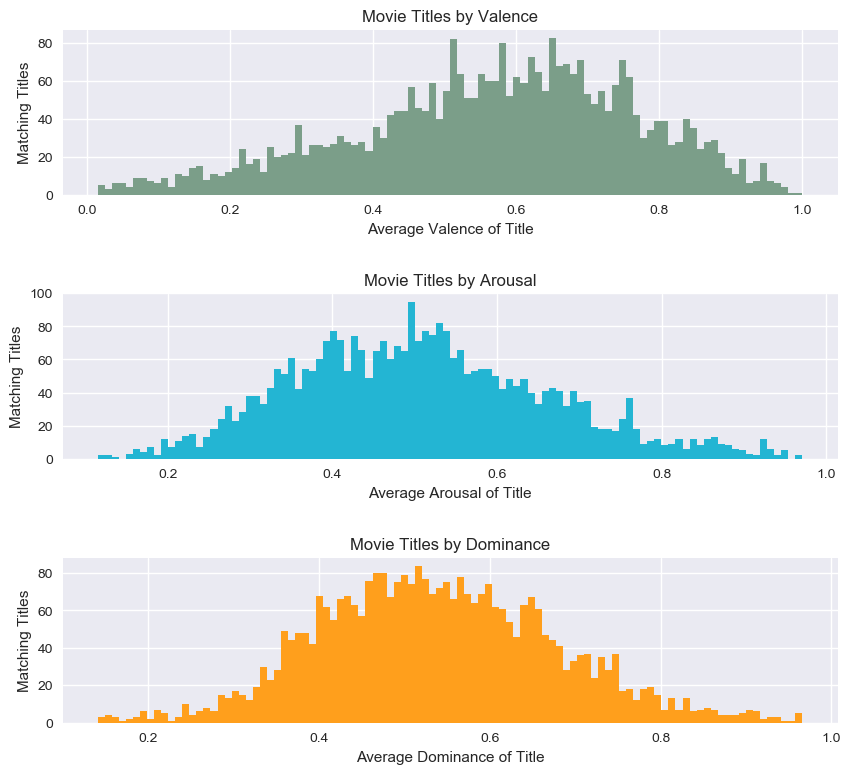
\includegraphics[scale=0.8]{Movie_titles_by_vad}
    Here we have a graph

    \begin{appendices}
        \section{Graphs}
        Figures of graphs are going to go here.
        \section{Something else}
        Things that are not graphs will go here.
    \end{appendices}
\end{document}
